\documentclass[10pt, titlepage]{article}

\usepackage[margin=1in]{geometry}
\usepackage{fancyhdr}
\usepackage{amsfonts}
\usepackage{amsmath}
\usepackage{amssymb}
\usepackage{booktabs}
\usepackage{tikz}
\usepackage{float}
\usepackage{tikz}
\usepackage{pgfplots}


\makeatletter
\setlength{\@fptop}{0pt}
\makeatother

\title{\normalsize PLUS Session Worksheet \\[1em] \Large \textit{MATH 1554:} Linear Algebra}
\author{Covering lessons: 6.1 -- 6.3}
\date{Summer 2023}

% ------- Set up header -------
\renewcommand{\sectionmark}[1]{\markright{#1}} % from https://tex.stackexchange.com/a/317393/227665
\pagestyle{fancy}
\fancyhead[L]{Summer 2023}
\fancyhead[C]{\textit{(6.1), (6.2), \& (6.3)}}
\fancyhead[R]{\textbf{\thepage}}
% -------------------------------------------------------

% ------- Set up Main Idea box environment -------
\newcounter{mainideas}
\setcounter{mainideas}{1}
\newcommand{\mainidea}{\textbf{Main Idea \#\themainideas \stepcounter{mainideas}}}
\setlength\fboxsep{1em}
%\newcommand{\midea}[2]{\begin{center}\fbox{\parbox{#1}{\centering \mainidea #2}} \end{center}} % Could be environment but I couldn't bother

% The way this works is that the savebox collects whatever was between the minipage and the end of it, then in the last line of the definition of the environment
% we regurgigate whatever was collected into an fbox which we center.
\newsavebox{\mybox}
\newenvironment{mideea}[1]
{%
\begin{lrbox}{\mybox}%
	\begin{minipage}{#1\textwidth}
		{\centering \mainidea \par}

}
{\end{minipage}\end{lrbox}\begin{center}\fbox{\usebox{\mybox}}\end{center}}
% -------------------------------------------------------

% ------- Set up activity environment -------
\newcounter{question}
\setcounter{question}{1}
\newenvironment{newquestion}
{
	\noindent\textbf{Question \thequestion}
}
{
\stepcounter{question}
\par
}
% -------------------------------------------------------


% ------- Set up math stuff -------
\renewcommand{\vec}[1]{\mathbf{#1}}
\DeclareMathOperator{\vspan}{Span}
\DeclareMathOperator{\row}{row}
\DeclareMathOperator{\col}{col}
\DeclareMathOperator{\colspace}{Col}
\DeclareMathOperator{\nullspace}{Nul}
\DeclareMathOperator{\rank}{rank}
% -------------------------------------------------------

% ------- Set up circle -------
\newcommand{\bubble}{\tikz[baseline=-0.625ex]\draw[radius=0.5em, fill=white] (0,0) circle;}
\newcommand{\dbubble}{\tikz[baseline=-0.625ex]\draw[radius=0.5em, fill=black] (0,0) circle;}
% -------------------------------------------------------

\begin{document}
\maketitle

\section{\centering Dot Product, Length, and Orthogonality (6.1)}
	\begin{newquestion}
		For the following statements, answer \textit{true} if the statement is always true, and \textit{false} otherwise.
		\begin{table}[!h]
			\centering
			\begin{tabular}{c@{\hspace{2.5em}}cp{0.75\textwidth}}
				true & false & \\
				\specialrule{\lightrulewidth}{0.25em}{1.25em}
				\bubble & \bubble & For any scalar \(c \in \mathbb{R}\), \(\|c\vec{v}\| = c\|\vec{v}\|\). \\[0.75em]
				\bubble & \bubble & If \(\vec{u} \cdot \vec{v} = 0\), then \(\|\vec{v} - \vec{u}\| = \|\vec{v} + \vec{u}\|.\)\\[0.75em]
				\bubble & \bubble & If \(\vec{y} \in \mathbb{R}^n\) is orthogonal to some \(\vec{z} \in W\), 
							      where \(W\) is a subspace of \(\mathbb{R}^n\), then \(\vec{y} \in W^\perp\). \\[0.75em]
				\bubble & \bubble & If \(A \in \mathbb{R}^{10 \times 12}\) and \(\rank A = 6\), then \(\dim (\nullspace A^T) = 6\).\\[0.75em]
				\bottomrule
			\end{tabular}
		\end{table}
	\end{newquestion}

\section{\centering Orthogonal Sets (6.2)}

	\begin{newquestion}
		Answer the following statements with \textit{possible} if the statement \emph{could} be true.
		\begin{table}[!h]
			\centering
			\begin{tabular}{c@{\hspace{2.5em}}cp{0.75\textwidth}}
				possible & impossible & \\
				\specialrule{\lightrulewidth}{0.25em}{1.25em}
				\bubble & \bubble & A vector whose projection onto a subspace \(W\) is itself. \\[0.75em]
				\bubble & \bubble & A non-zero vector whose projection into a subspace is the zero vector.\\[0.75em]
				\bubble & \bubble & 2 orthogonal planes in \(\mathbb{R}^3\). \\[0.75em]
				\bubble & \bubble & Two vectors that form a linearly dependent set but also an orthogonal set. \\[0.75em]
				\bubble & \bubble & \(A\) is orthogonal matrix and \(B\) is an orthogonal matrix as well, but \(AB\) isn't. \\[0.75em]
				\bottomrule
			\end{tabular}
		\end{table}
	\end{newquestion}

	\begin{newquestion}
		Let \(A = \small \begin{pmatrix}1/\sqrt{2} & 0 & -1/\sqrt{2}\\ 0 & 1 & 0\\ 1/\sqrt{2} & 0 & 1/\sqrt{2}\end{pmatrix}\) and 
		\(\vec{v} = \begin{pmatrix}1 \\ 0 \\ 3\end{pmatrix}\). Find \(\|A\vec{v}\|\).
	\end{newquestion}

\section{\centering Orthogonal Decomposition \& Projection (6.3)}
	\begin{newquestion}
		Answer the following statements with \textit{possible} if the statement \emph{could} be true.
		\begin{table}[!h]
			\centering
			\begin{tabular}{c@{\hspace{2.5em}}cp{0.75\textwidth}}
				possible & impossible & \\
				\specialrule{\lightrulewidth}{0.25em}{1.25em}
				\bubble & \bubble & The projection of a vector onto a subspace depends on the basis of the subspace. \\[0.75em]
				\bubble & \bubble & A nonzero vector \(\vec{v}\) with \(\vec{v} \in W\) and \(\vec{v} \in W^\perp\). \\[0.75em]
				\bubble & \bubble & A vector \(\vec{y}\) such that \(\vec{y} - \operatorname{proj}_W \vec{y} \notin W^\perp\). \\[0.75em]
				\bottomrule
			\end{tabular}
		\end{table}
	\end{newquestion}

	\begin{newquestion}
		\begin{enumerate}
			\item Find the distance between \(\begin{pmatrix}2 \\ 3\end{pmatrix}\) and the subspace formed by the span of the vector 
			\(\begin{pmatrix}1 \\ 0\end{pmatrix}\).
			\item Find the distance between \(\begin{pmatrix}2 \\ 3\end{pmatrix}\) and the vector \(\begin{pmatrix}1 \\ 0\end{pmatrix}\).
		\end{enumerate}
	\end{newquestion}

\fancyhead[C]{\textit{Solutions}}

\section{Solutions to Section 1}
	\begin{table}[!h]
		\centering
		\begin{tabular}{c@{\hspace{2.5em}}cp{0.75\textwidth}}
			true & false & \\
			\specialrule{\lightrulewidth}{0.25em}{1.25em}
			\bubble & \dbubble & For any scalar \(c \in \mathbb{R}\), \(\|c\vec{v}\| = c\|\vec{v}\|\). \\[0.75em]
			\dbubble & \bubble & If \(\vec{u} \cdot \vec{v} = 0\), then \(\|\vec{v} - \vec{u}\| = \|\vec{v} + \vec{u}\|.\)\\[0.75em]
			\bubble & \dbubble & If \(\vec{y} \in \mathbb{R}^n\) is orthogonal to some \(\vec{z} \in W\), 
						      where \(W\) is a subspace of \(\mathbb{R}^n\), then \(\vec{y} \in W^\perp\). \\[0.75em]
			\bubble & \dbubble & If \(A \in \mathbb{R}^{10 \times 12}\) and \(\rank A = 6\), then \(\dim (\nullspace A^T) = 6\).\\[0.75em]
			\bottomrule
		\end{tabular}
	\end{table}

\subsection{Justifications}
\paragraph{Justification to \textit{Q1}} It should be \(\lvert c\rvert \|\vec{v}\|\).

\paragraph{Justification to \textit{Q2}} Calculate \(\|\vec{v} - \vec{u}\|^2\) and \(\|\vec{v} + \vec{u}\|^2\). Since the norm always defines a positive value, 
							we know that if the squares are equal, then so are the square roots.

\begin{align*}
	\|\vec{v} - \vec{u}\|^2 &= (\vec{v} - \vec{u})^T(\vec{v} - \vec{u}) \\
				           &= \vec{v}^T\vec{v} - \vec{v}^T\vec{u} - \vec{u}^T\vec{v} + \vec{u}^T\vec{u} \\
                                           &= \|\vec{v}\|^2 + \|\vec{u}\|^2
\end{align*}

\begin{align*}
	\|\vec{v} + \vec{u}\|^2 &= (\vec{v} + \vec{u})^T(\vec{v} + \vec{u}) \\
				           &= \vec{v}^T\vec{v} + \vec{v}^T\vec{u} + \vec{u}^T\vec{v} + \vec{u}^T\vec{u} \\
                                           &= \|\vec{v}\|^2 + \|\vec{u}\|^2
\end{align*}

Since \(\|\vec{v} - \vec{u}\|^2 = \|\vec{v} + \vec{u}\|^2\), \(\|\vec{v} - \vec{u}\| = \|\vec{v} + \vec{u}\|\).

\paragraph{Justification to \textit{Q3}} The vector \(\vec{y}\) has to be orthogonal to \emph{every} vector in \(W\), not just \emph{some}.

\paragraph{Justification to \textit{Q4}} \(\dim (\nullspace A^T) = 4\).


\section{Solutions to Section 2}
	\begin{table}[!h]
		\centering
		\begin{tabular}{c@{\hspace{2.5em}}cp{0.75\textwidth}}
			possible & impossible & \\
			\specialrule{\lightrulewidth}{0.25em}{1.25em}
			\dbubble & \bubble & A vector whose projection onto a subspace \(W\) is itself. \\[0.75em]
			\dbubble & \bubble & A non-zero vector whose projection into a subspace is the zero vector.\\[0.75em]
			\bubble & \dbubble & 2 orthogonal planes in \(\mathbb{R}^3\). \\[0.75em]
			\dbubble & \bubble & Two vectors that form a linearly dependent set but also an orthogonal set. \\[0.75em]
			\bubble & \dbubble & \(A\) is orthogonal matrix and \(B\) is an orthogonal matrix as well, but \(AB\) isn't. \\[0.75em]
			\bottomrule
		\end{tabular}
	\end{table}
	
	\subsection{Justifications}
	\paragraph{Justification to Q1} For any vector \(\vec{y} \in W\), where \(W\) is a subspace, \(\operatorname{proj}_W \vec{y} = \vec{y}\).
	\paragraph{Justification to Q2} Any orthogonal vector to \(W\) will have a projection equal to the zero vector.
	\paragraph{Justification to Q3} The dimension of orthogonal complements have to add up to the dimension of the vector space, which is 3 in this case.
	\paragraph{Justification to Q4} \((AB)(AB)^T = A(BB^T)A^T = AA^T = I.\) So \(AB\) is orthogonal as well.

	\subsection{Solution to Question 3}
	Note that the matrix \(A\) is orthogonal. Hence, \(\|A\vec{v}\| = \|\vec{v}\|.\) We see that \(\|\vec{v}\| = \sqrt{10} = \|A\vec{v}\|\).

\section{Solutions to Section 3}
	\begin{table}[!h]
		\centering
		\begin{tabular}{c@{\hspace{2.5em}}cp{0.75\textwidth}}
			possible & impossible & \\
			\specialrule{\lightrulewidth}{0.25em}{1.25em}
			\bubble & \dbubble & The projection of a vector onto a subspace depends on the basis of the subspace. \\[0.75em]
			\bubble & \dbubble & A nonzero vector \(\vec{v}\) with \(\vec{v} \in W\) and \(\vec{v} \in W^\perp\). \\[0.75em]
			\bubble & \dbubble & A vector \(\vec{y}\) such that \(\vec{y} - \operatorname{proj}_W \vec{y} \notin W^\perp\). \\[0.75em]
			\bottomrule
		\end{tabular}
	\end{table}

	\subsection{Justifications}
	\paragraph{Justification to Q1} The projection of a vector onto a subspace is unique and does not depend on the basis of the subspace but rather the 
						      subspace itself.
	\paragraph{Justification to Q2} If \(\vec{v} \in W\) and \(\vec{v} \in W^\perp\), then \(\vec{v} \cdot \vec{v} = 0\). The only vector with this property is the
						      zero vector.
	\paragraph{Justification to Q3} Refer back to how orthogonal decomposition works.


	\subsection{Solution to Question 5}
	\begin{enumerate}
		\item \textbf{3}. A picture.
		\begin{figure}[!h]
			\centering
			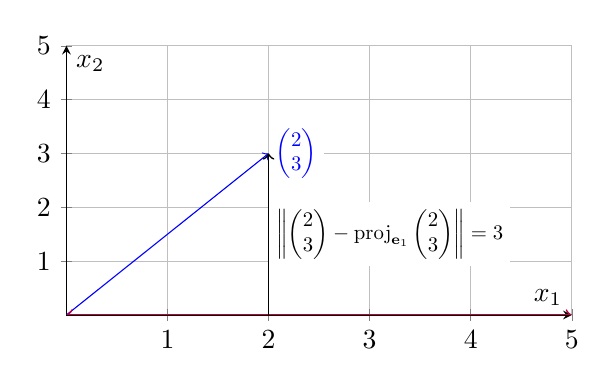
\begin{tikzpicture}
				\begin{axis}[height = 5cm, width=8cm, axis lines = middle, xlabel = {\(x_1\)}, ylabel = {\(x_2\)}, xtick distance = 1, ytick distance = 1, xmin=0, xmax=5, ymin=0, ymax=5, grid=major]
					\plot[blue, ->]coordinates {(0, 0) (2, 3)} node[right, fill=white, scale=0.75] {\(\begin{pmatrix}2 \\ 3\end{pmatrix}\)};
					\plot[<->, semithick, purple, domain=0:5] ({x}, {0});
					\draw[semithick, ->] (axis cs: 2, 0) -- node[right, fill=white, scale=0.75] {\(\biggl\|\begin{pmatrix}2 \\ 3\end{pmatrix} - \operatorname{proj}_{\vec{e}_1} \begin{pmatrix}2 \\ 3\end{pmatrix}\biggr\| = 3\)} (axis cs: 2, 3) ;
				\end{axis}
			\end{tikzpicture}
		\end{figure}
		\item \(\mathbf{\sqrt{10}}\). Another picture.
		\begin{figure}[!t]
			\centering
			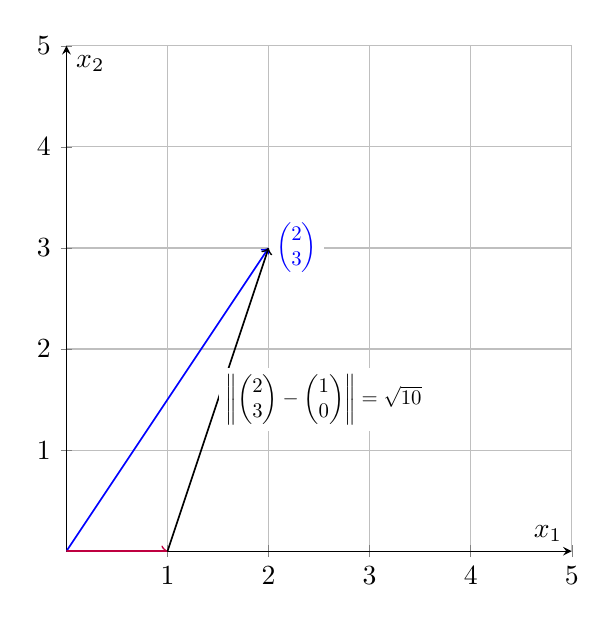
\begin{tikzpicture}
				\begin{axis}[height = 8cm, width=8cm, axis lines = middle, xlabel = {\(x_1\)}, ylabel = {\(x_2\)}, xtick distance = 1, ytick distance = 1, xmin=0, xmax=5, ymin=0, ymax=5, grid=major]
					\plot[blue, ->, semithick]coordinates {(0, 0) (2, 3)} node[right, fill=white, scale=0.75] {\(\begin{pmatrix}2 \\ 3\end{pmatrix}\)};
					\plot[purple, ->, semithick] coordinates {(0, 0) (1, 0)};
					\draw[black, ->, semithick] (axis cs: 1, 0) -- node[right, fill=white, scale=0.75] {\(\biggl\|\begin{pmatrix}2 \\ 3\end{pmatrix} - \begin{pmatrix}1 \\ 0\end{pmatrix}\biggr\| = \sqrt{10}\)} (axis cs: 2, 3);
				\end{axis}
			\end{tikzpicture}
		\end{figure}
	\end{enumerate}
\end{document}
